\section{Structure générale}
Vigilate est une solution composé de 3 programmes différents :\\
\begin{itemize}
\item Un site web\\
\item Un scanner\\
\item Un backend\\
\end{itemize}
Vigilate pourra optionnellement être distribué sur une vm.\\
\section{Le site web}
Le site web servira à la personnalisation des alertes. On pourra choisir quels programmes suivre. On pourra aussi choisir un niveau de criticité minimum par programme  pour être prévenu. Le site permettra aussi de choisir le ou les moyens par lesquels on veut être prévenu lors de la découverte d’une vulnérabilité (mail, sms ou notifications sur le site). Le site web enverra ces données au backend via l’api pour qu’il mette à jour la base de donnée.\\
Le site web utilisera django côté serveur, la communication avec l’api se feras donc en python. Cotés client il utiliseras angularJS afin de mieux interagir avec l'utilisateur\\

\section{Le scanner de programme}
Le scanner de programmes est là par soucis de simplicité d’utilisation, ce sera un programme en python (donc portable) qui récupérera la liste des programmes installés et les enverra au backend via l’api pour mettre à jour la base de donnée. Le scanner pourra être lancé manuellement ou planifié pour s’exécuter régulièrement (par exemple une fois par semaine).\\

\section{Le Backend}
Le backend sera le coeur de vigilate. C’est un programme qui récupérera les cve dès leurs sortie via le flux rss du site cve.mitre.org. Une fois récupérées il les stockera dans la base de données et regardera si un des clients utilise ce programme, si c’est le cas il vérifiera ensuite si la version est vulnérable. Puis il ira voir si le niveau de criticité est égale ou supérieur à celui précisé par le client via le site web, si c’est le cas il préviendra le client par tous les moyens que celui-ci aura choisi.\\
Le backend recevra aussi  les informations du scanneur et les stockera dans une base de donnée.\\
Le backend hébergera aussi l’api de vigilate, cette api permettra au backend de communiquer avec le scanner et le site web, elle récupérera leur requêtes et fera les modifications nécessaires dans la base de données. L’api permettra de modifier la liste de programmes installés et leurs versions ainsi que de changer les préférences (niveau de criticité et moyen de contact).\\
Il y aura aussi une API publique. Cette API sera utilisable par client qui souhaite intégrer Vigilate à leur solution. On peut par exemple imaginer un hébergeur qui propose le service vigilate à ses clients afin qu’il puissent monitorer la sécurité des programmes qu’ils utilisent.\\
Le backend seras lui aussi codé en python, les API public et interne seront de type REST. Ce qui permettra une utilisation simple et clair avec angularjs.\\


\section{La vm}
Pour finir Vigilate offrira optionnellement une vm.\\
Les serveurs de Vigilate contiendront la liste des programmes de chaque utilisateur. Ces informations peuvent être sensibles si elles appartiennent à des entreprises ayant besoin d’un grand niveau de sécurité. Vigilate en mode VM répond à ce problème.
\\
Ce sera machine virtuelle prête à fonctionner qui contiendra le site web et le backend de vigilate. Un système de mises à jour permettra à la vm d’avoir les composants de vigilate constamment à jours sans avoir à la réinstaller. La vm restera connecté à notre API de façon chiffrée et sécurisée, afin de récupérer les nouvelles vulnérabilités qui sont publiées. C’est la VM qui se charge de comparer l’information avec ses données locales pour envoyer ou non les alertes de sécurité.
\\
Vigilate en mode VM permet aux entreprises critiques de garder en local les informations sensibles de sécurité de leur infrastructure. Aucune information sortira du réseau, en effet la VM utilise seulement un flux réseau descendant pour les mises à jour.


\section{Cas d’utilisation}
\begin{figure}[!h]
  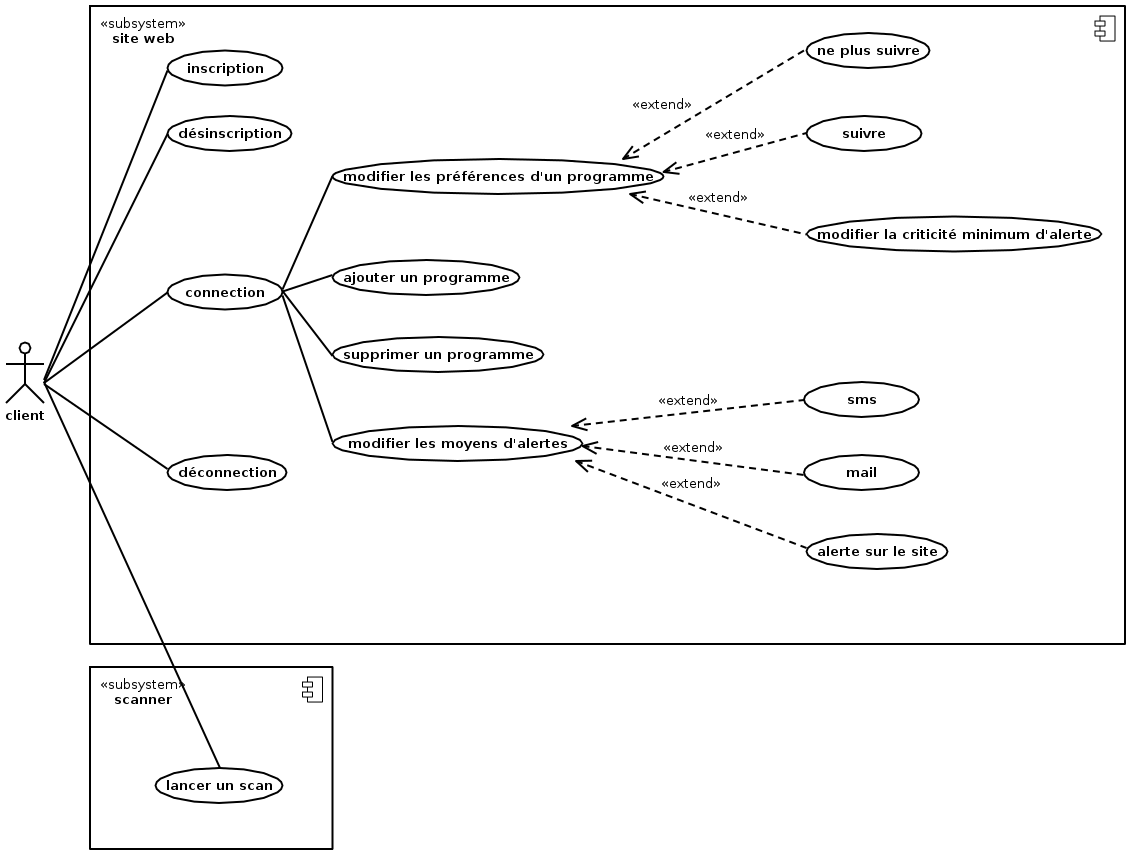
\includegraphics[width=18cm]{uml1.png}
\end{figure}
\begin{figure}[!h]
  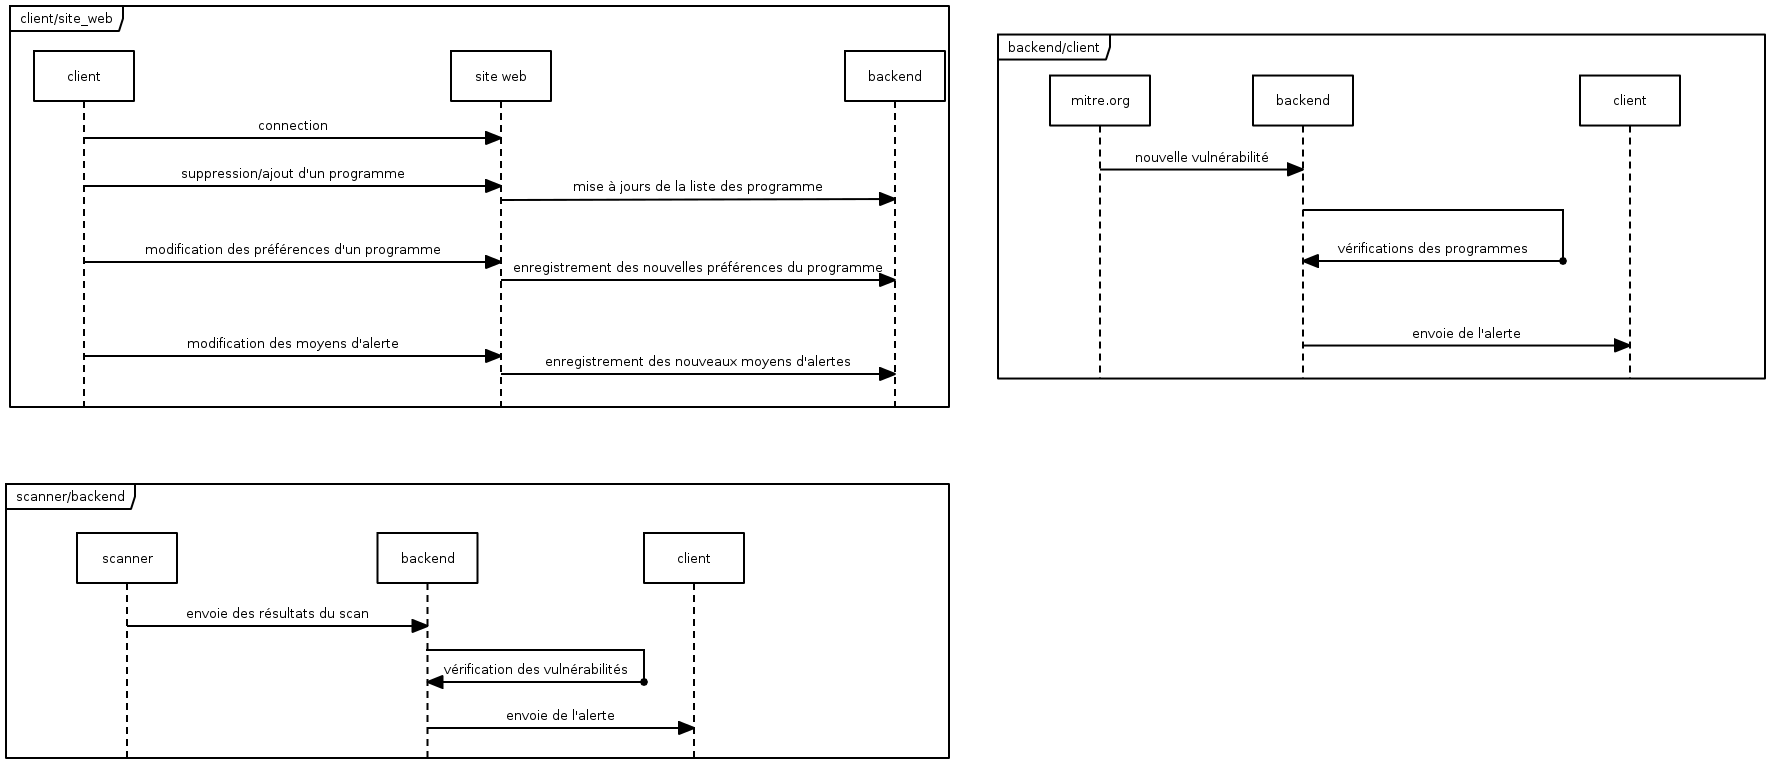
\includegraphics[width=18cm]{uml2.png}
\end{figure}
